%%%%%%%%%%%%%%%%%%%%%%%%%%%%%%%%%%%%%%%%%%%%%%%%%%%%%%%%%%%%%%%%%%%%%%%%%%%%%%%%
\section{Motivos}
\label{sec:Motivo}
\index{Música!Motivos}
\index{Música!Motif}
\index{Música!Motiv}

Na literatura sobre música podemos achar  termos, motiv (em alemão) ou motif (em inglês),
para designar ao que no português chamaríamos como motivo \cite[pp. 984]{latham2008diccionario}.
Um motivo é uma unidade melódica curta que se repete ao longo de uma composição musical \cite[pp. 545]{apel1969harvard},
esta tem como intenção proporcionar integração, relação, coerência, lógica, 
compreensão e fluidez ao discurso musical \cite[pp. 984]{latham2008diccionario};
sendo estes usados como elementos básicos para a construção
de temas e linhas melódicas \cite[pp. 984]{latham2008diccionario}.

Os motivos são geralmente mais pequenos que um tema ou uma frase,
podendo ter tamanhos tão pequenos quanto só duas notas,
se estas forem o suficientemente representativas \cite[pp. 545]{apel1969harvard}.

%Los *Leitmotiven (motivos principales) de Wagner son el ejemplo más común
%de ideas musicales concisas que además de proporcionar un elemento 
%de estabilidad en la continuidad musical, contribuyen directamente al desarrollo coherente
%de la acción dramática  \cite[pp. 545]{apel1969harvard}.

\begin{example}
Um exemplo muito interessante de uso de motivos pode ser visto na sinfonia n. 5, op. 67, 
de Ludwig van Beethoven.
Na Figura \ref{fig:10Symphony5Op67}, podemos ver os 10 primeiros compassos da sinfonia,
numa versão simplificada que usa só 3 instrumentos, 2 violinos e uma viola.
Nesse fragmento é identificável o motivo nos dois primeiros compassos,
com um conjunto de notas correspondentes a ``sol~sol~sol~mi$\flat$''.
Nos seguintes 3 compassos, o mesmo motivo é usado, 
mas este sofre uma diminuição de 1 tom na altura de todas as notas, 
além de que a última nota musical sofre um amento na sua duração. 
Finalmente nos últimos 5 compassos, cada instrumento por separado sofre uma diferente mutação do motivo;
o violino 1, usa o motivo com um ganho de 8 semitons e um pequeno aumento da ultima nota;
a viola, usa o motivo com um ganho de 13 semitons e um aumento considerável da última nota; e
o violino 2, usa o motivo com um importante aumento na longitude da última nota.
\end{example}


\begin{figure}[!h]
  \centering
    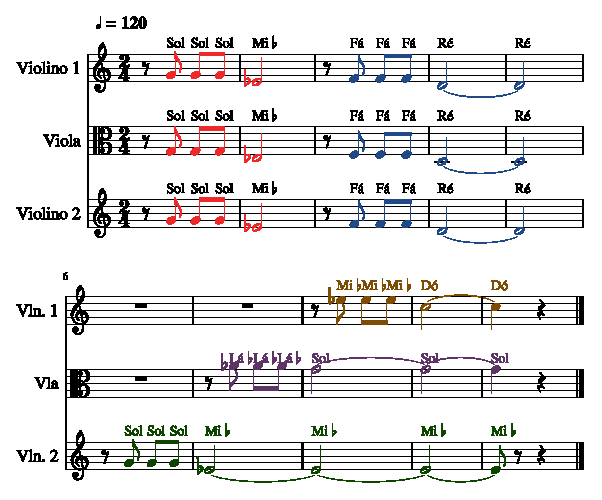
\includegraphics[width=\workboxsize]{chapters/cap-musica-composer/Symphony5Op67-out-1.eps}
\caption{Dez compassos da sinfonia no. 5, op. 67, de Ludwig van Beethoven.}
\label{fig:10Symphony5Op67}
\end{figure}

~


\begin{example}
Na música ``Tico-tico no fubá'' de Zequinha de Abreu, podemos achar exemplos do uso de motivos. 
Na Figura \ref{fig:Tico-tico_no_fuba-1}, temos 5 compassos desta música,
numa versão que usa só 1 instrumentos (um bandolim).
Nesse fragmento é identificável o motivo nos dois primeiros compassos, 
nas 6 primeiras notas musicais, ``mi~ré~mi~fá~mi~lá$\#$''.
imediatamente depois o motivo se repete, porém mudando a ultima nota ate um ``sol$\#$'';
finalmente o motivo volta a parecer, só que além da modificação na altura na ultima nota a um ``ré'',
a duração é encurtada e mais 6 notas musicais são agregadas.
Esta recorrência no uso deste motivo e outros podem ser vistos ao longo de toda a peça musical;
assim, animamo ao leitor a procurar e ouvir a música completa, e tentar identificar o motivo e suas mutações. 
\end{example}

\begin{figure}[!h]
  \centering
    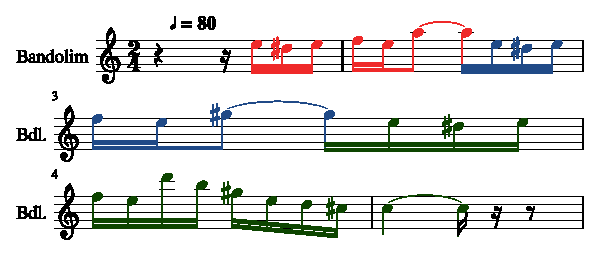
\includegraphics[width=\workboxsize]{chapters/cap-musica-composer/Tico-tico_no_fuba-1.eps}
\caption{Cinco compassos da música ``Tico-tico no fubá'' de Zequinha de Abreu.}
\label{fig:Tico-tico_no_fuba-1}
\end{figure}

~

